\documentclass[12pt,letterpaper]{article}

\usepackage[utf8]{inputenc}
\usepackage[T1]{fontenc}
\usepackage{amsmath}
\usepackage{amsfonts}
\usepackage{amssymb}
\usepackage{amsthm}
\usepackage[left=2cm,right=2cm,top=2cm,bottom=2cm,headheight=22pt]{geometry}
\usepackage{fancyhdr}
\usepackage{setspace}
\usepackage{lastpage}
\usepackage{graphicx}
\usepackage{caption}
\usepackage{subcaption}
\usepackage{paralist}

\theoremstyle{definition}
\newtheorem{question}{Question}

\begin{document}

%Paramètres de mise en forme des paragraphes selon les normes françaises
\setlength{\parskip}{1ex plus 0.5ex minus 0.2ex}
\setlength{\parindent}{0pt}

%Paramètres relatifs aux en-têtes et pieds de page.
\pagestyle{fancy}
\lhead{Theron J Hitchman}
\chead{\Large First Exam}
\rhead{Fall 2013}
\lfoot{\emph{Math and Decision Making}}
\cfoot{}
\rfoot{\emph{\thepage\ of \pageref{LastPage}}}

\section*{Instructions}
Please write your responses, with any supporting diagrams, on the separate pieces of white paper provided.  You have one hour to complete this exam. I expect you to explain yourself clearly whenever possible.

\section*{The Examination Questions}

\begin{question}
In class, we discussed \emph{picture hanging puzzles}. Here is a variant we did not discuss directly. Describe a solution and why it works.

Find a way to wrap the wire hanger for a picture frame around four nails so that 
\begin{compactitem}
\item If any subset of three nails is removed, the picture will fall down; but,
\item If any subset of only one or two nails is removed, the picture will remain hanging on the wall.
\end{compactitem}
\end{question}

\vspace{.5in}

%\begin{question}
%Describe clearly what we mean when we call two knots ``the same." We often use the term \emph{ambient isotopy}, but what does that mean?
%
%Write as if describing the idea to a friend who is not in this class, but might take it next semester.
%\end{question}

%\vspace{.5in}

\begin{question}
The two knots whose planar projections are drawn below in Figure \ref{fig:rm-pic} are equivalent knots. Show how to realize this with a short sequence of Reidemeister moves.
\begin{figure}[h!]
    \centering
    \begin{subfigure}{.3\textwidth}
        \centering
        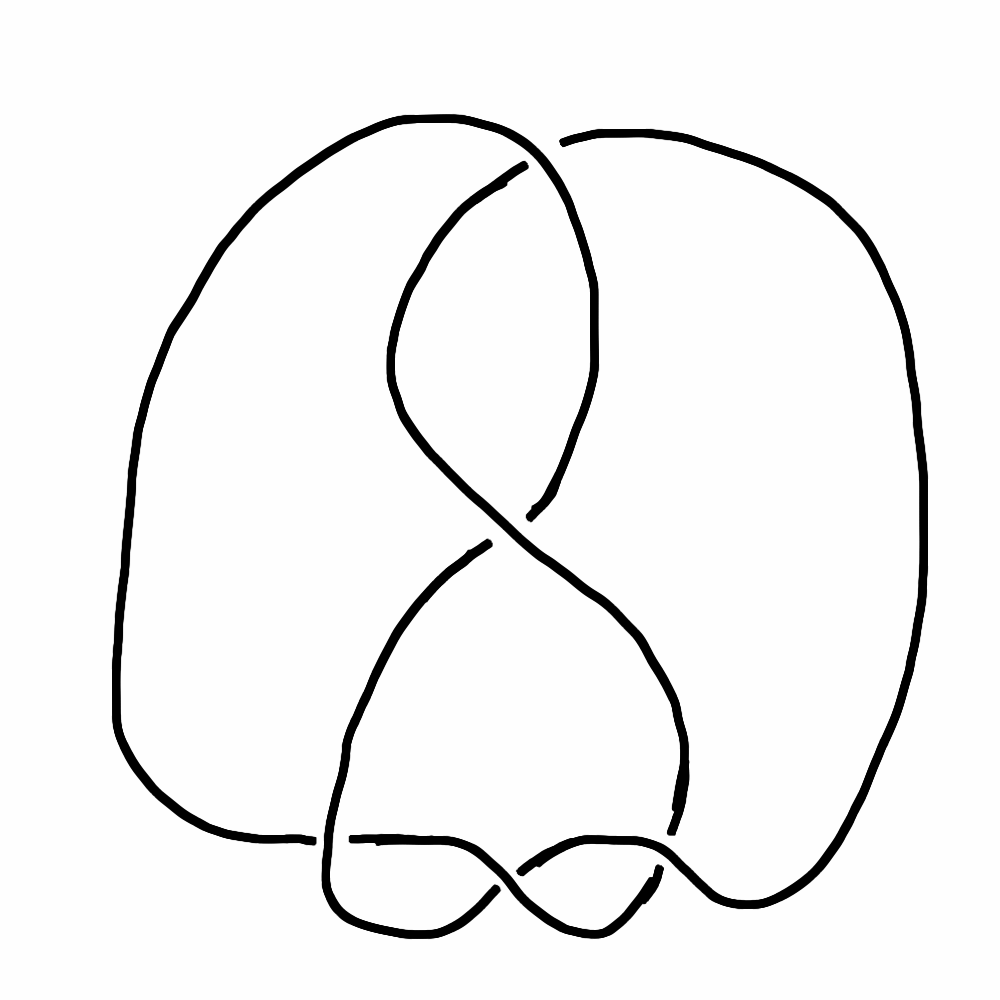
\includegraphics[width=\textwidth]{knotpics/exercise2-1.png}
        \caption{Knot A}
    \end{subfigure}
    \hspace{1cm}
    \begin{subfigure}{.3\textwidth}
        \centering
        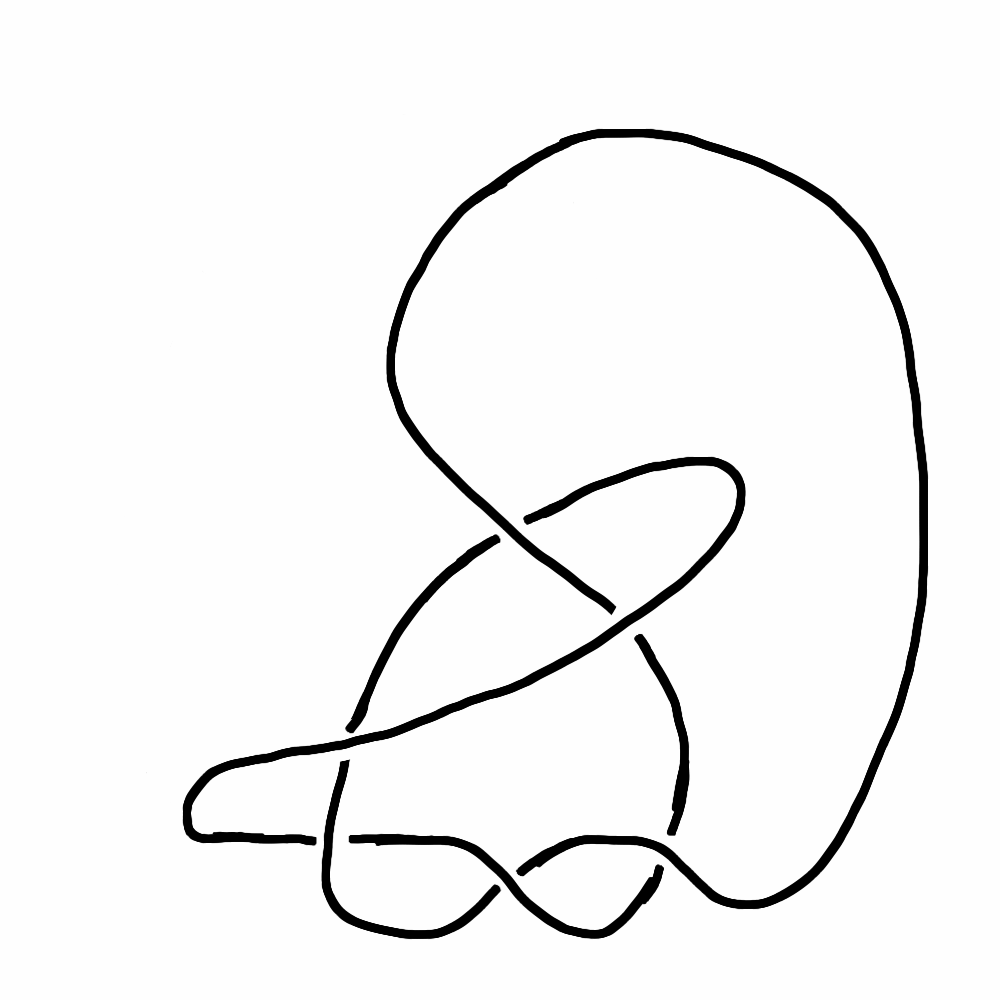
\includegraphics[width=\textwidth]{knotpics/exercise2-2.png}
        \caption{Knot B}
    \end{subfigure}
    \caption{Equivalent knots}
    \label{fig:rm-pic}
\end{figure}
\end{question}

\vspace{.5cm}

\begin{question}\label{question:classify}
On the back of this page, you will find planar projection diagrams for seven truly different, non-equivalent links.
Use the invariants we have computed to explain how you know for sure that no pair of these can represent equivalent links.
\end{question}

\clearpage

\section*{Diagrams for Question \ref{question:classify}}

\begin{figure}[h!]
    \centering
    \begin{subfigure}{.3\textwidth}
        \centering
        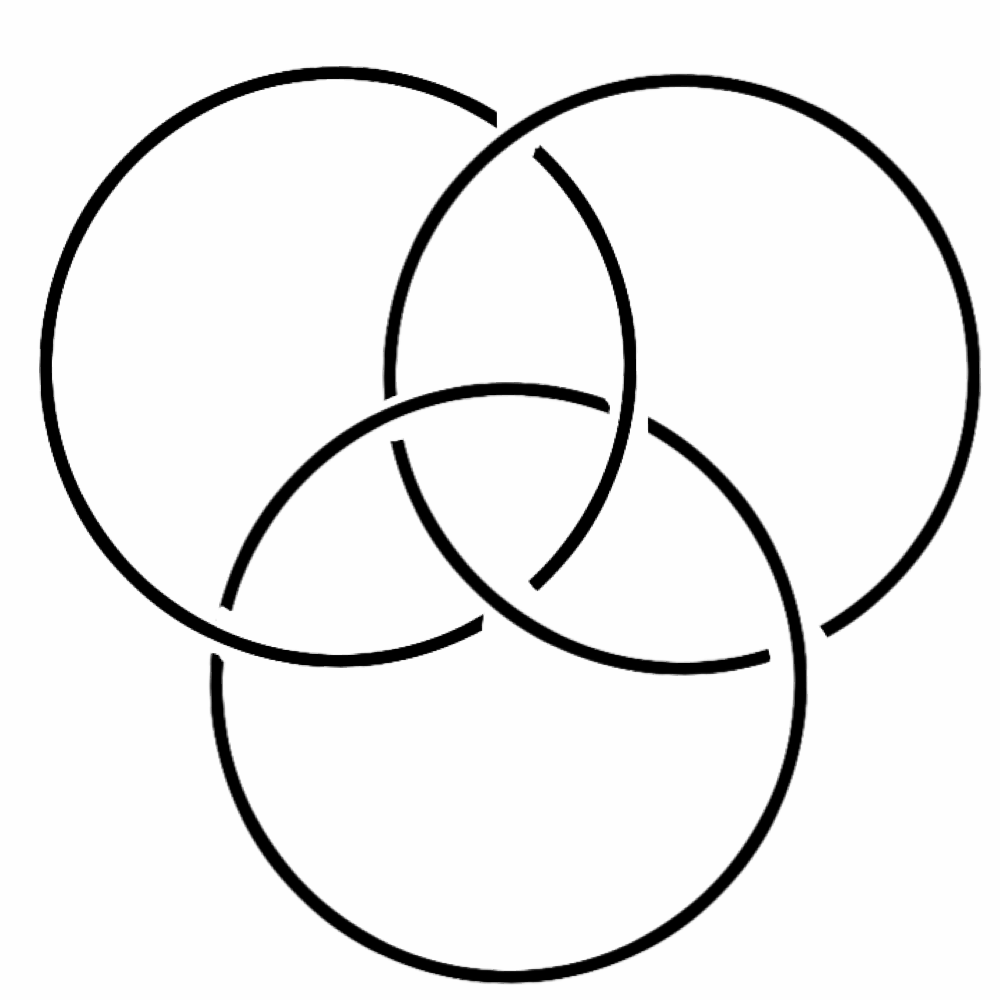
\includegraphics[width=\textwidth]{knotpics/borromean.png}
        \caption{Link A}
    \end{subfigure}
    \hspace{.5cm}
    \begin{subfigure}{.3\textwidth}
        \centering
        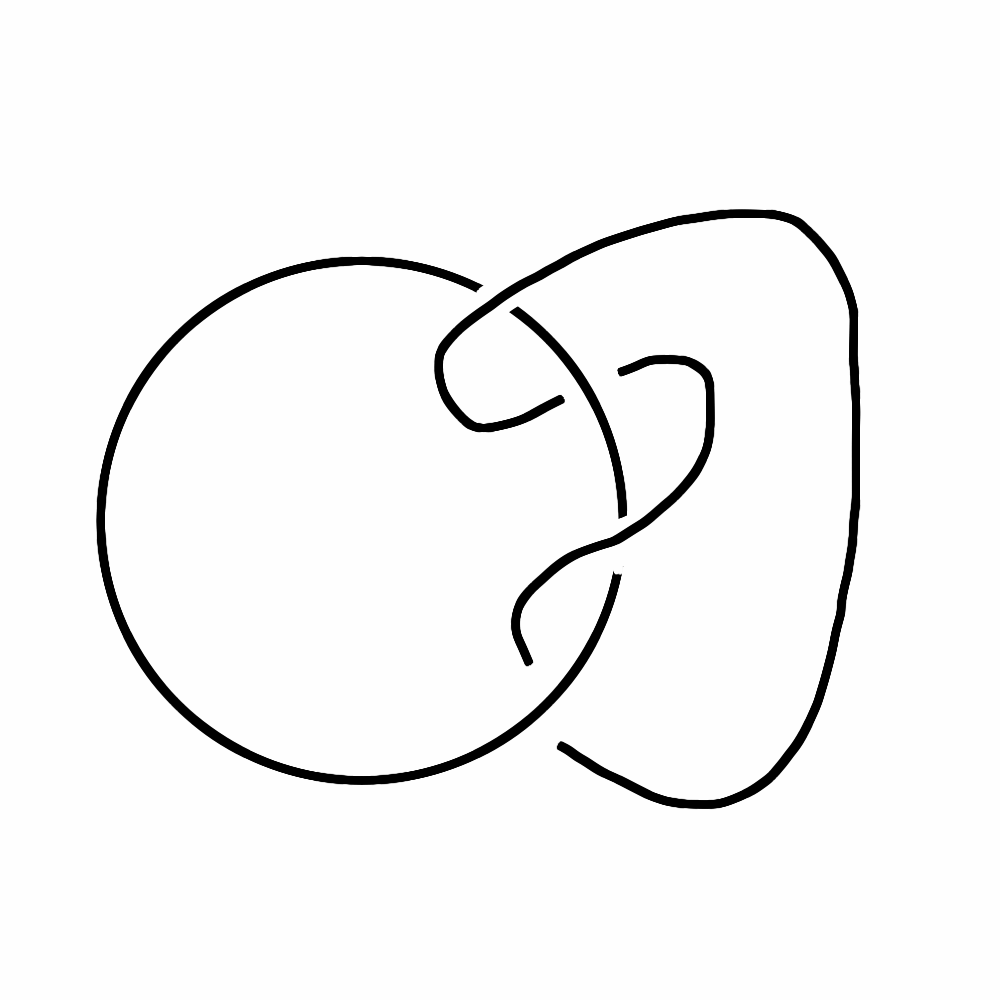
\includegraphics[width=\textwidth]{knotpics/lno2.png}
        \caption{Link B}
    \end{subfigure}
    \hspace{.5cm}
    \begin{subfigure}{.3\textwidth}
        \centering
        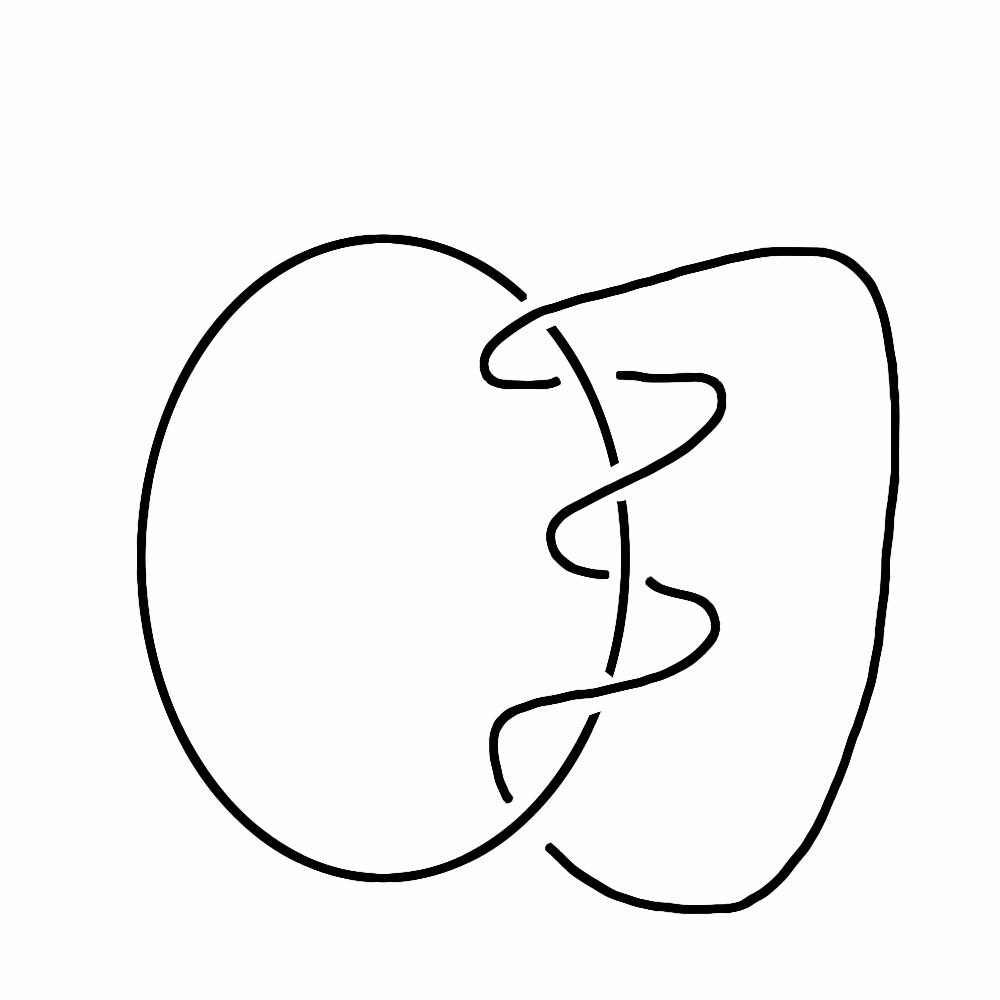
\includegraphics[width=\textwidth]{knotpics/lno3.png}
        \caption{Link C}
    \end{subfigure}
    
    \begin{subfigure}{.4\textwidth}
        \centering
        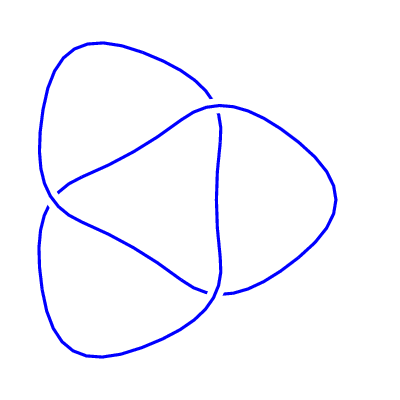
\includegraphics[width=\textwidth]{knotpics/3_1mirror.png}
        \caption{Link D}
    \end{subfigure}
    \hspace{.5cm}
    \begin{subfigure}{.4\textwidth}
        \centering
        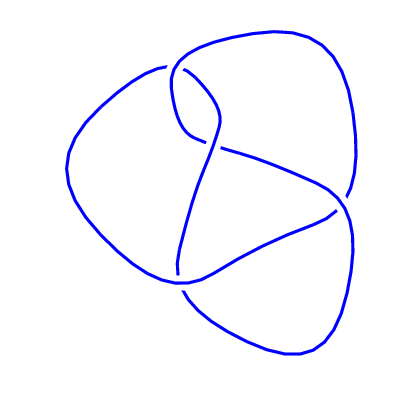
\includegraphics[width=\textwidth]{knotpics/4_1.png}
        \caption{Link E}
    \end{subfigure}
    
    \begin{subfigure}{.4\textwidth}
        \centering
        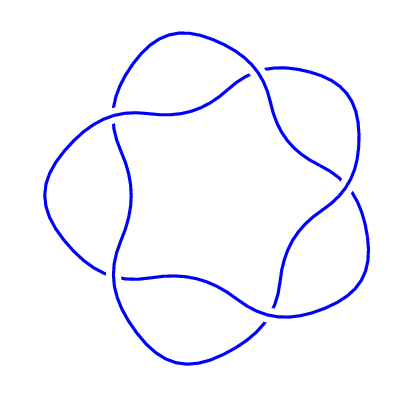
\includegraphics[width=\textwidth]{knotpics/5_1.png}
        \caption{Link F}
    \end{subfigure}
    \hspace{.5cm}
    \begin{subfigure}{.4\textwidth}
        \centering
        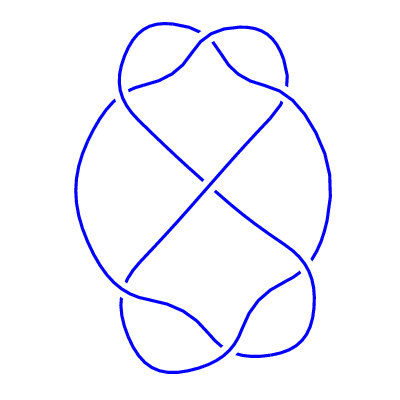
\includegraphics[width=\textwidth]{knotpics/7_4.png}
        \caption{Link G}
    \end{subfigure}
    \caption{Some non-equivalent links}
\end{figure}



\clearpage









\end{document}
%sagemathcloud={"zoom_width":100}